% DISC-IP-003  (JMFK)
% Invention disclosure: variable projection fitting of dark adaptation
% recovery curves in the RapiDA dark adaptometer.
% Compile with xelatex. Figure files fig1-model-curve.tex,
% fig2-varpro-loop.tex, fig3-grid-search.tex must sit alongside this file.
\documentclass[11pt,a4paper]{article}
\usepackage[margin=25mm]{geometry}
\usepackage{iftex}
\ifpdftex
  \usepackage[T1]{fontenc}
  \usepackage[utf8]{inputenc}
  \usepackage{helvet} % closest stock match to Helvetica Neue under pdflatex
\else
  \usepackage{fontspec}
  \IfFontExistsTF{Helvetica Neue}
    {\setmainfont{Helvetica Neue}}
    {\relax} % fall back to the default font if Helvetica Neue is absent
\fi
\usepackage{amsmath}
\usepackage{tikz}
\usetikzlibrary{positioning, arrows.meta}
\usepackage{pgfplots}
\pgfplotsset{compat=1.18}
\usepackage{booktabs}
\usepackage{fancyhdr}
\usepackage[framemethod=tikz]{mdframed}
\usepackage{enumitem}

% ---- figure colour definitions (required by all three figures) ----
\definecolor{coneC}{HTML}{D85A30}
\definecolor{rodC}{HTML}{534AB7}
\definecolor{tealC}{HTML}{0F6E56}
\definecolor{grayC}{HTML}{5F5E5A}

% ---- document identity ----
\newcommand{\docid}{DISC-IP-003}
\newcommand{\docversion}{v0.2 draft}
\newcommand{\docdate}{14 August 2026}

% ---- headers and footers ----
\pagestyle{fancy}
\fancyhf{}
\fancyhead[L]{\small MuMac Ltd}
\fancyhead[R]{\small \docid\ \docversion}
\fancyfoot[L]{\footnotesize Confidential: prepared for the purpose of
  obtaining legal advice}
\fancyfoot[R]{\small Page \thepage}
\renewcommand{\headrulewidth}{0.4pt}

% ---- placeholder box for content to be completed ----
\newmdenv[linecolor=coneC, linewidth=1pt, roundcorner=4pt,
  backgroundcolor=coneC!6, frametitle={To complete before submission},
  frametitlefont=\small\bfseries]{todo}

\begin{document}

% ================= title block =================
\begin{center}
{\LARGE Invention disclosure}\\[2mm]
{\Large Variable projection fitting of dark adaptation\\
recovery curves}\\[6mm]
\begin{tabular}{ll}
\toprule
Document ID & \docid \\
Version & \docversion \\
Date & \docdate \\
Author & JMFK \\
Company & MuMac Ltd \\
Status & Draft for review \\
\bottomrule
\end{tabular}
\end{center}

\vspace{4mm}
\noindent\textbf{Version history}

\noindent\begin{tabular}{llll}
\toprule
Version & Date & Author & Change \\
\midrule
v0.1 & 13 August 2026 & JMFK & Initial draft \\
v0.2 & 14 August 2026 & JMFK & Novelty basis, disclosure record,\\
     &                &      & reduction to practice, grid bounds \\
\bottomrule
\end{tabular}

\vspace{6mm}
\section{Document purpose and scope}
This document discloses a method for fitting dark adaptation recovery
curves, as implemented in the RapiDA dark adaptometer, for the purpose of
seeking advice on patentability. It is intended for MuMac's patent attorney
and, in abridged form, for the MuMac board. This document and its contents
are confidential.

\section{Background}
Dark adaptation, the recovery of visual sensitivity after exposure to a
bright light, is a functional biomarker for age-related macular
degeneration (AMD). Rod-mediated recovery is measurably delayed in early
AMD, often before structural changes are visible, which makes the shape of
the recovery curve clinically valuable for early detection.

The RapiDA dark adaptometer measures this recovery. The participant is
exposed to a controlled bleach and their detection threshold is then
sampled repeatedly in darkness. The clinical output is not the raw
thresholds but the parameters of a model fitted to them; the quality,
speed, and repeatability of that fit determine the quality of the device's
output.

\section{The model}
We model the recovery of visual sensitivity during dark adaptation with
the function
\begin{equation}
\text{thres}(t) = ct + cc\,e^{-t/\tau} + S2\,(t-\alpha)\,H(t-\alpha),
\label{eq:model}
\end{equation}
where:
\begin{itemize}[nosep]
\item $\text{thres}(t)$ is the measured threshold at time $t$ after bleach;
\item $ct$ is the cone threshold, the plateau to which cone-mediated
  sensitivity recovers;
\item $cc$ is the cone coefficient, the amplitude of the cone recovery
  component;
\item $\tau$ is the cone time constant;
\item $S2$ is the slope of the second (rod-mediated) component of
  recovery;
\item $\alpha$ is the rod--cone break, the time at which rod recovery
  begins;
\item $H(t-\alpha)$ is the Heaviside step function, equal to $0$ for
  $t < \alpha$ and $1$ for $t \geq \alpha$.
\end{itemize}
The term $(t-\alpha)H(t-\alpha)$ is therefore a ramp: it is zero before
the rod--cone break and changes linearly with slope $S2$ after it.
Figure~\ref{fig:model} shows the model and its components.

\begin{figure}[ht]
\centering
% fig1-model-curve.tex  (JMFK)
% Dark adaptation model: cone branch, cone threshold ct, rod branch from alpha.
% Requires: tikz, pgfplots (\pgfplotsset{compat=1.18}), arrows.meta.
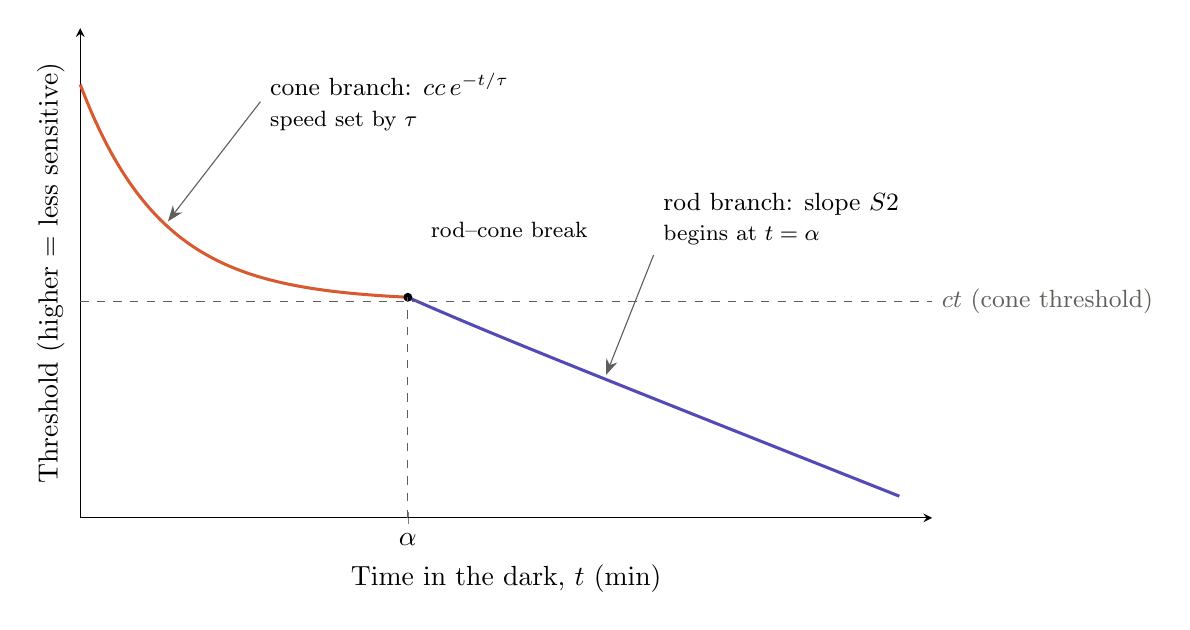
\begin{tikzpicture}
% ---- model parameters: edit these, everything else follows ----
\def\pCT{1.0}      % cone threshold
\def\pCC{1.0}      % cone coefficient
\def\pTAU{2.5}     % cone time constant (min)
\def\pALPHA{10}    % rod-cone break (min)
\def\pSTWO{-0.06}  % rod slope (negative = threshold falls)
\def\pTMAX{25}     % end of plotted time range (min)
% ---- callout layout: x positions of the two arrow targets ----
\def\xConePt{2.6}
\def\xRodPt{16}
% ---- derived quantities (do not edit) ----
\pgfmathsetmacro{\yBreak}{\pCT + \pCC*exp(-\pALPHA/\pTAU)}
\pgfmathsetmacro{\yConePt}{\pCT + \pCC*exp(-\xConePt/\pTAU)}
\pgfmathsetmacro{\yRodPt}{\pCT + \pCC*exp(-\xRodPt/\pTAU) + \pSTWO*(\xRodPt-\pALPHA)}
\pgfmathsetmacro{\yMax}{(\pCT + \pCC)*1.13}
\pgfmathsetmacro{\xMax}{\pTMAX + 1}
\begin{axis}[
  width=124mm, height=78mm,
  axis lines=left,
  xlabel={Time in the dark, $t$ (min)},
  ylabel={Threshold (higher $=$ less sensitive)},
  xmin=0, xmax=\xMax, ymin=0, ymax=\yMax,
  ytick=\empty,
  xtick={\pALPHA}, xticklabels={$\alpha$},
  clip=false,
  every axis plot/.append style={line width=1.1pt},
]
% cone-dominated portion (full model, rod term zero before alpha)
\addplot[coneC, domain=0:\pALPHA, samples=120]
  {\pCT + \pCC*exp(-x/\pTAU)};
% rod-dominated portion (full model including the ramp)
\addplot[rodC, domain=\pALPHA:\pTMAX, samples=120]
  {\pCT + \pCC*exp(-x/\pTAU) + \pSTWO*(x-\pALPHA)};
% rod-cone break marker
\fill (axis cs:\pALPHA,\yBreak) circle[radius=1.6pt];
% ct plateau guide
\draw[dashed, grayC] (axis cs:0,\pCT) -- (axis cs:\xMax,\pCT)
  node[anchor=west, font=\small] {$ct$ (cone threshold)};
% alpha guide
\draw[dashed, grayC] (axis cs:\pALPHA,0) -- (axis cs:\pALPHA,\yBreak);
\node[anchor=west, font=\footnotesize]
  at (axis cs:{\pALPHA+0.4},{\yBreak+0.31}) {rod--cone break};
% cone branch callout
\node[anchor=west, font=\small, align=left] (conelbl)
  at (axis cs:{0.55*\pALPHA},{0.85*\yMax})
  {cone branch: $cc\,e^{-t/\tau}$\\ \footnotesize speed set by $\tau$};
\draw[grayC, shorten >=1.5pt, -{Stealth[length=2mm]}]
  (conelbl.west) -- (axis cs:\xConePt,\yConePt);
% rod branch callout
\node[anchor=west, font=\small, align=left] (rodlbl)
  at (axis cs:{\pALPHA+7.5},{0.61*\yMax})
  {rod branch: slope $S2$\\ \footnotesize begins at $t=\alpha$};
\draw[grayC, shorten >=1.5pt, -{Stealth[length=2mm]}]
  (rodlbl.south west) -- (axis cs:\xRodPt,\yRodPt);
\end{axis}
\end{tikzpicture}

\caption{The dark adaptation model. The cone branch (orange) decays with
time constant $\tau$ towards the cone threshold $ct$; at the rod--cone
break $\alpha$ the rod branch (purple) begins, changing with slope $S2$.
Parameter values are illustrative.}
\label{fig:model}
\end{figure}

\section{The problem with conventional fitting}
Equation~\eqref{eq:model} has five unknown parameters. The conventional
approach is to estimate all five simultaneously by iterative nonlinear
least squares. This has three practical defects for a clinical device:
\begin{enumerate}[nosep]
\item \textbf{Starting guesses.} Iterative solvers require initial values
  for all five parameters. Poor guesses cause failed or wrong fits, and
  choosing good guesses on noisy clinical data is itself unsolved.
\item \textbf{Local minima.} The five-dimensional error surface has
  multiple minima. The solver can converge to a plausible-looking but
  wrong answer, and there is no internal signal that it has done so.
\item \textbf{Irreproducibility.} Different starting guesses, solver
  settings, or library versions can produce different fitted parameters
  from identical data. For a medical device this is a regulatory and
  repeatability problem, not merely an inconvenience.
\end{enumerate}
These concerns are not hypothetical. MuMac's current instruments produce
real-time parameter estimates during the test using gradient descent, and
a single fit can require up to 20{,}000 iterations. The iteration count
is data-dependent and unbounded in principle, which makes worst-case
timing on device hardware difficult to guarantee.

\section{The method}
\subsection{Rewriting the model in a familiar form}
Most STEM scientists are familiar with the equation of a straight line,
\begin{equation}
y = c + mx,
\end{equation}
where $y$ is the response, $x$ is the independent variable, $c$ is the
intercept and $m$ is the gradient. Fitting this line to data by ordinary
least squares (OLS) has a closed-form solution: no iteration, no starting
guesses.

Our aim is to show that, under one condition, our model has exactly the
same character. We want to reach the form
\begin{equation}
\mathbf{Y} = a + \mathbf{B}\,\mathbf{F}(\mathbf{x}),
\end{equation}
where $\mathbf{Y}$ is the vector of participant responses, $\mathbf{x}$ is
the vector of response time stamps, $a$ is an intercept, $\mathbf{F}$ is a
set of basis functions evaluated at those time stamps, and $\mathbf{B}$ is
a vector of coefficients. This is the straight-line equation with the
single term $mx$ replaced by a sum of curved terms.

Suppose the two nonlinear parameters, $\tau$ and $\alpha$, are held fixed.
Then define two basis functions:
\begin{equation}
f_1(\mathbf{x}) = e^{-\mathbf{x}/\tau}, \qquad
f_2(\mathbf{x}) = (\mathbf{x}-\alpha)\,H(\mathbf{x}-\alpha).
\end{equation}
The model becomes
\begin{equation}
\mathbf{Y} = ct + cc\,f_1(\mathbf{x}) + S2\,f_2(\mathbf{x})
           = a + \mathbf{B}\,\mathbf{F}(\mathbf{x}),
\end{equation}
with $a = ct$ playing the role of the intercept $c$, and
$\mathbf{B} = (cc,\ S2)$. This is a linear model. Every quantity we do not
know appears only as an intercept or a multiplying coefficient. Those
familiar with OLS will recognise that the best-fitting $a$ and
$\mathbf{B}$ can be computed together in closed form, exactly as for the
straight line.

\subsection{The variable projection loop}
The full model is nonlinear only through $\tau$ and $\alpha$. Variable
projection (VarPro) exploits this structure:
\begin{enumerate}[nosep]
\item For any candidate pair $(\tau, \alpha)$, the intercept and
  coefficients $(ct, cc, S2)$ are obtained analytically by least squares.
  They are never searched for.
\item The optimisation therefore reduces from a five-parameter nonlinear
  search to a two-parameter search over $(\tau, \alpha)$ alone.
\end{enumerate}
Figure~\ref{fig:loop} shows the loop.

\begin{figure}[ht]
\centering
% fig2-varpro-loop.tex  (JMFK)
% Variable projection search loop: only (tau, alpha) is searched;
% ct, cc, S2 are solved in closed form at every candidate.
% Requires: tikz with libraries positioning, arrows.meta.
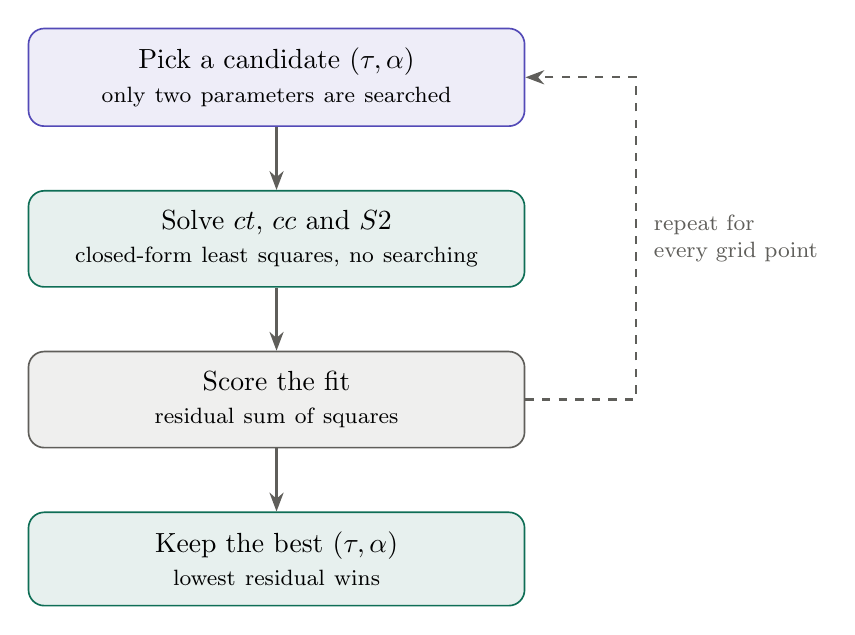
\begin{tikzpicture}[
  node distance=8mm,
  box/.style={rectangle, rounded corners=2mm, draw, line width=0.6pt,
              text width=58mm, align=center, inner sep=2.5mm},
  searched/.style={box, draw=rodC, fill=rodC!10},
  solved/.style={box, draw=tealC, fill=tealC!10},
  neutral/.style={box, draw=grayC, fill=grayC!10},
  arr/.style={-{Stealth[length=2.4mm]}, line width=0.8pt, grayC},
]
\node[searched] (pick)
  {Pick a candidate $(\tau,\alpha)$\\ \footnotesize only two parameters are searched};
\node[solved, below=of pick] (solve)
  {Solve $ct$, $cc$ and $S2$\\ \footnotesize closed-form least squares, no searching};
\node[neutral, below=of solve] (score)
  {Score the fit\\ \footnotesize residual sum of squares};
\node[solved, below=of score] (keep)
  {Keep the best $(\tau,\alpha)$\\ \footnotesize lowest residual wins};
\draw[arr] (pick) -- (solve);
\draw[arr] (solve) -- (score);
\draw[arr] (score) -- (keep);
% return path of the outer loop
\draw[arr, dashed] (score.east) -- ++(14mm,0) |- (pick.east)
  node[pos=0.25, right, font=\footnotesize, align=left, xshift=1mm]
  {repeat for\\ every grid point};
\end{tikzpicture}

\caption{The variable projection search loop. Only the two nonlinear
parameters $(\tau,\alpha)$ are searched (purple); the intercept and
coefficients $(ct, cc, S2)$ are obtained analytically at every candidate
(teal).}
\label{fig:loop}
\end{figure}

Because the two-dimensional $(\tau,\alpha)$ space is small, it can be
searched exhaustively over a grid (Figure~\ref{fig:grid}). Every cell of
the grid costs a single closed-form solve, so the entire space is
evaluated, the global minimum over the grid is found by construction, and
identical data always produce identical fitted parameters.

\begin{figure}[ht]
\centering
% fig3-grid-search.tex  (JMFK)
% Exhaustive grid search over the (tau, alpha) plane. Cell shade = fit error
% (darker = better); the star marks the lowest residual. Every cell costs one
% closed-form solve, so the search is deterministic and reproducible.
% Requires: tikz with library arrows.meta. Shading is synthetic/illustrative.
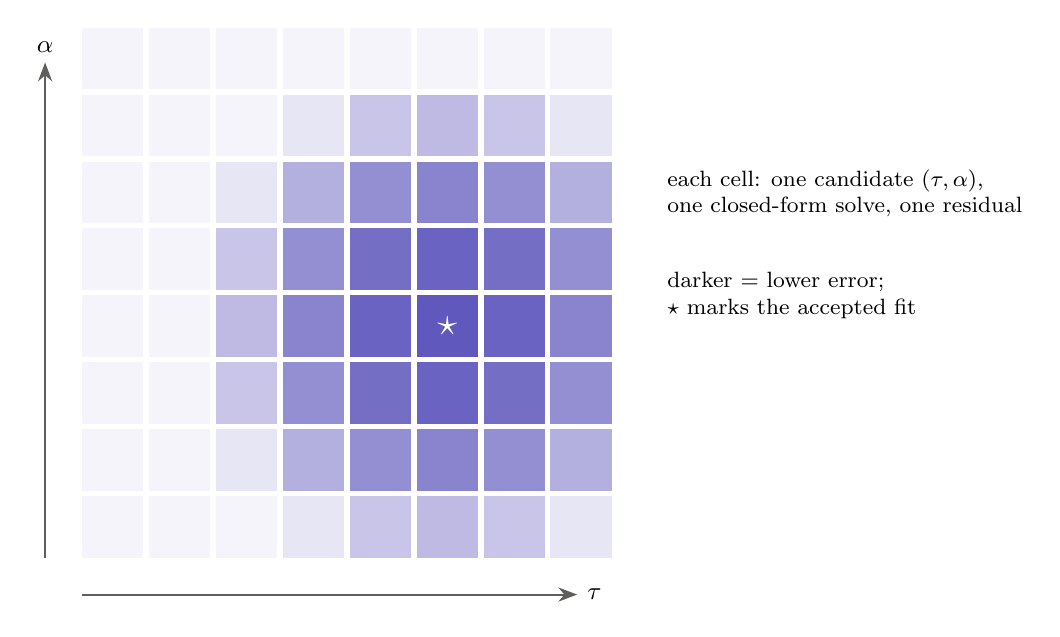
\begin{tikzpicture}[x=8.5mm, y=8.5mm]
% ---- grid parameters: edit these, everything else follows ----
\def\gN{8}          % grid is gN x gN cells
\def\gBestTau{5}    % column of the best cell (0-based)
\def\gBestAlpha{3}  % row of the best cell (0-based)
\def\gShadeMax{92}  % shade percentage at the minimum (darkest)
\def\gShadeSlope{6.0} % how fast shade fades with error distance
\def\gShadeMin{6}   % shade floor at the grid edges (lightest)
% ---- derived quantities (do not edit) ----
\pgfmathtruncatemacro{\gLast}{\gN - 1}
\pgfmathsetmacro{\gAxisEnd}{\gN - 0.6}
\foreach \i in {0,...,\gLast}{
  \foreach \j in {0,...,\gLast}{
    \pgfmathsetmacro{\err}{(\i-\gBestTau)*(\i-\gBestTau)
                         + (\j-\gBestAlpha)*(\j-\gBestAlpha)}
    \pgfmathsetmacro{\pct}{max(\gShadeMin, \gShadeMax - \gShadeSlope*\err)}
    \fill[rodC!\pct] (\i, \j) rectangle ++(0.92, 0.92);
  }
}
% best cell
\node[white, font=\Large\bfseries]
  at ({\gBestTau+0.46}, {\gBestAlpha+0.46}) {$\star$};
% axes
\draw[-{Stealth[length=2.4mm]}, grayC, line width=0.7pt]
  (0,-0.55) -- (\gAxisEnd,-0.55) node[right, font=\small, black] {$\tau$};
\draw[-{Stealth[length=2.4mm]}, grayC, line width=0.7pt]
  (-0.55,0) -- (-0.55,\gAxisEnd) node[above, font=\small, black] {$\alpha$};
% legend
\node[anchor=west, font=\footnotesize, align=left]
  at ({\gN+0.6}, {0.68*\gN})
  {each cell: one candidate $(\tau,\alpha)$,\\ one closed-form solve, one residual};
\node[anchor=west, font=\footnotesize, align=left]
  at ({\gN+0.6}, {0.49*\gN})
  {darker $=$ lower error;\\ $\star$ marks the accepted fit};
\end{tikzpicture}

\caption{Exhaustive search over the $(\tau,\alpha)$ plane. Each cell costs
a single closed-form solve, so the whole grid is evaluated and the fit is
deterministic and reproducible. Shading is illustrative.}
\label{fig:grid}
\end{figure}

\section{Novelty over prior art}
Known prior art, stated for completeness:
\begin{itemize}[nosep]
\item Variable projection as a general numerical method: Golub and
  Pereyra (1973) and the subsequent literature.
\item The dark adaptation model of Equation~\eqref{eq:model} and its
  variants, established in the visual science literature.
\item Existing dark adaptometers and their published fitting approaches.
\end{itemize}

MuMac does not claim novelty in the variable projection method itself, nor
in the dark adaptation model. The asserted novelty lies in the
application: the use of variable projection, with an exhaustive grid
search over the two nonlinear parameters, to fit the two-branch dark
adaptation model within a clinical dark adaptometer. Specifically:
\begin{itemize}[nosep]
\item the recognition that the clinical model of
  Equation~\eqref{eq:model} separates into two nonlinear and three linear
  parameters, and the exploitation of that structure in a measurement
  instrument;
\item the replacement of an in-device iterative fit, currently requiring
  up to 20{,}000 gradient descent iterations for real-time parameter
  estimates during the test, with a bounded, fixed-cost computation:
  one closed-form solve per grid cell, giving a worst-case run time that
  is known in advance;
\item the use of an exhaustive grid over $(\tau,\alpha)$, made affordable
  by the closed-form inner solve, so that the fit is deterministic:
  identical measurement data always yield identical clinical parameters,
  a property that can be stated and verified for regulatory purposes;
\item the elimination of starting guesses and per-patient solver tuning,
  enabling unattended operation by non-specialist users on noisy clinical
  data.
\end{itemize}
The method will be implemented in the forthcoming RapiDA Mk3 instrument,
where it replaces the gradient descent fit of the current models. The
method has no built-in adaptive mechanism: its real-time output is a
predictive model of the participant's recovery, and the operator may
curtail the test once satisfied with the quality of the responses. The
fit therefore shortens testing through informed operator judgement rather
than automatic control.
Whether an application of a known numerical method to a new technical
purpose is patentable is a question for the attorney; the technical
effects of the application (real-time in-test fitting with bounded,
known-in-advance cost, deterministic tuning-free clinical output, and
operator-informed test curtailment) should be central to that assessment.

The grid bounds are clinically derived. Operational experience shows that
the cone time constant $\tau$ is always below two minutes. The range of
the rod--cone break $\alpha$ is contingent on the flash intensity used by
the test protocol; a fitted $\alpha$ beyond five minutes indicates that
the subject received a flash well below the intensity required for
rate-limited recovery of rod photoreceptor function, and flags an
inadequate bleach rather than a physiological result. The upper bound on
$\alpha$ therefore doubles as a built-in validity check on the bleaching
stage of the test. The grid over $(\tau,\alpha)$ is bounded by physiology
and protocol, and the exhaustive search covers the full clinically
relevant range: the accepted fit is the best fit over all physiologically
plausible parameter pairs, not merely the best that a heuristic search
happened to find.

\section{Advantages and commercial significance}
\begin{itemize}[nosep]
\item \textbf{Speed and bounded cost.} The search space collapses from
  five dimensions to two, and the fit becomes a fixed number of
  closed-form solves in place of up to 20{,}000 data-dependent gradient
  descent iterations. Worst-case run time is known in advance, which
  matters for real-time use on device hardware.
\item \textbf{Robustness.} No starting guesses are required for the
  linear parameters, removing a common source of fitting failure on noisy
  clinical data.
\item \textbf{Reproducibility.} The exhaustive grid gives a deterministic
  fit: identical inputs always yield identical outputs, a property that
  can be stated and verified in regulatory submissions.
\item \textbf{No operator tuning.} The method has no per-patient solver
  settings, supporting use by non-specialist operators.
\item \textbf{Shorter tests.} The real-time predictive model lets the
  operator curtail the test once the responses are of sufficient quality,
  reducing test duration for the participant without loss of fitted
  parameters.
\end{itemize}

\begin{todo}
Market context paragraph to be supplied by the co-directors (IJM, WP):
AMD prevalence, the early-detection opportunity, and where a protected
fitting method sits in MuMac's IP position alongside the hardware.
\end{todo}

\section{Reduction to practice}
The method is implemented and working. The implementation is held in a
private GitHub repository under the inventor's control; no person other
than the inventor is aware of the codebase, and access is restricted
accordingly. Early implementations were developed and run on the
inventor's local development machine (macOS). The large-scale numerical
experiment described in Section~9.3, planned to investigate the validity
of the methodology, will be run on a novel RISC-V device.

The repository's commit history provides contemporaneous, timestamped
evidence of development and is reproduced in Annex~B. The repository was
created on 3~August~2026. The variable projection fit, implemented under
the working name ``profile least squares'' (a standard synonym for the
same technique: the linear parameters are profiled out of the
optimisation), was introduced in commit \texttt{dd5ea31} on
6~August~2026 at 00:12~BST, and a working fitting routine for the
exponential decay component via profiled least squares was in place by
commit \texttt{f755c3e} on 6~August~2026 at 12:31~BST. The method was
therefore first implemented and working on or about 6~August~2026.
Subsequent commits prepare the codebase for the discrimination study,
which is the numerical experiment of Section~9.3.

For completeness of the timeline: implementation (6~August~2026) precedes
the Bluesky post recorded in Section~9.2 (12~August~2026), and this
disclosure document (13~August~2026) follows both.

Early development was tested against both real measured recovery data and
several instances of simulated data. The simulated data serve verification
(known ground-truth parameters recovered correctly); the real data
demonstrate the method working on measurement noise of clinical
character.

\section{Inventorship and disclosure history}
\subsection{Inventorship}
The method described in this document was conceived and implemented
solely by Dr Jeremiah MF Kelly (MuMac Ltd). No other person contributed
to the inventive concept. The inventor has not been employed by the
University of Manchester for more than ten years, and under the spin-out
arrangements the University assigned all intellectual property to MuMac
Ltd. The method was conceived and developed entirely within MuMac Ltd,
and ownership rests with the company.

\subsection{Disclosure history}
The method has not been described in any paper, conference talk, poster,
investor document, grant application, or website content. It has been
disclosed in private to the following individuals:
\begin{itemize}[nosep]
\item the inventor's spouse;
\item Prof.\ Ian J Murray, director of MuMac Ltd;
\item Mr Bill Pigg, non-executive director of MuMac Ltd, engaged under
  contract with an existing non-disclosure agreement.
\end{itemize}
None of these communications is believed to constitute a public
disclosure: the directors owe duties of confidence to the company, one is
additionally bound by an NDA, and the spousal communication was private.

One public statement exists and is listed for the attorney's assessment.
The inventor posted the following comment on the social network Bluesky:
\begin{quote}
``Well, I've spent ten years or more dealing with methods for analysing
non-linear models, only to find out about variable projection. All that
gradient descent and continuous function stuff is gone. Onward and
upward, I suppose.''
\end{quote}
The post does not describe the dark adaptation model, the application,
the exhaustive grid search, or any implementation detail, and is believed
to be non-enabling: it discloses at most that a well-known numerical
method was found useful on unspecified nonlinear modelling work. The
attorney should judge whether it has any bearing on novelty. Record of
the post, verified against the live page on 14 August 2026: posted from
the account @emkayoh.bsky.social on 12 August 2026 at 21:51 UTC, at\\
\texttt{\small https://bsky.app/profile/emkayoh.bsky.social/post/3msw4fxqk4s2m};\\
at the time of verification it had one like and one repost.

Two protective measures are in place: no further public comment on
fitting methods will be made, in any forum, until a filing decision has
been taken; and MuMac holds a copy of the University of Manchester IP
assignment, available for the attorney's file.

\subsection{Planned disclosures}
A large-scale numerical experiment is planned to investigate the validity
of the methodology, with the intention of publishing the results as a
monograph. The experiment itself is internal and discloses nothing; the
monograph, once published, would be a full enabling disclosure of the
method. The filing timetable should therefore be set ahead of the
monograph: a priority application must be on file before publication, and
the attorney should advise on the earlier steps too, since sharing a
manuscript with publishers or reviewers can itself carry disclosure risk
unless done under confidence. The monograph is an asset in this respect
as well as a constraint: published after filing, it would provide
independent, dated validation of the method without costing any rights.

\appendix
\section{Full mathematical treatment}
\begin{todo}
Full mathematical treatment to be written by JMFK: the design-matrix
formulation, the normal equations or QR-based solve used in the
implementation, grid resolution and bounds for $(\tau,\alpha)$, and
treatment of edge cases (no measurable break within the test window,
censored thresholds). Include references, beginning with Golub, G.H. and
Pereyra, V. (1973), SIAM Journal on Numerical Analysis 10(2), 413--432.
\end{todo}

\section{Repository commit history}
Commit history of the private implementation repository, oldest first,
generated with
\texttt{git log --reverse --date=iso}
and reproduced verbatim on 14~August~2026.
\begin{small}
\begin{verbatim}
2026-08-03 15:29:40 +0100  420e41a  first commit
2026-08-03 20:35:36 +0100  bcb8617  Initial commit
2026-08-05 21:49:25 +0100  7b19a8d  Initial commit
2026-08-06 00:12:35 +0100  dd5ea31  Introduce profile least-squares
                                    initialisation for P5c optimisation
2026-08-06 00:15:25 +0100  cd993fd  final comment 2026-08-06
2026-08-06 11:20:39 +0100  4ca5e79  Add discrimination and inference
                                    framework
2026-08-06 12:31:21 +0100  f755c3e  simplified function to fit
                                    exponentail decay via profiled
                                    least squares
2026-08-06 12:32:04 +0100  ba96f60  minor alterations to code base in
                                    preparation for the discrimantion
                                    study
\end{verbatim}
\end{small}
Commit messages are reproduced exactly as written, including original
spellings. Author timestamps are self-recorded; GitHub's server-side
records can corroborate them if required.

\end{document}